\chapter{Evaluation}
\label{chap:Evaluation}

\section{Product}

The final product turned out close to what we wanted to build. However, due to lack of time some features where changed to be easier and some features were dropped from this release.

We are happy with the way the user interface shows types and the way the type checker works. The behaviour and interaction with the user interface also turned out in alignment with our set requirements.

Our target audience included people who are familiar with Haskell. At this moment Viskell cannot completely satisfy these people. Missing features include a compact representation for larger programs, the ability to save and load programs and functionality for directly inputting Haskell code. Another thing is that there is no support for I/O or libraries besides Prelude. It is possible to add this functionality at a later point. But currently this made the audience shift towards a more educational use for beginning Haskell programmers.

We would have liked to make the program more useful for a large touch table where multiple users are interacting with the software at the same time. The circle menu would have been great for this purpose. Since our idea and prototype is described in this document we are confident that this can be implemented once this functionality is required.

\section{Process}

On the technical tools side, none of the members on the team had extensive experience with git \emph{and} GitHub \emph{and} Maven \emph{and} Travis, and some had never used either. It took quite a while for some to `get' the proposed workflow, and there was a lot of friction, many hours lost, and some frustration with those who struggled. Presentations on the subject helped, but some friction remained.

On a few occasions, we had difficulties planning sprints. Sprint goals and requirements either turned out to be vague at the end of the sprint, making it unclear or disputed whether or not we had completed them, or the goals were missed altogether. There also were times where we were not able to decide on how to implement certain features, which took up a lot of time.

The familiarity with the tools grew during the project, and all members became more comfortable with the tools. We also saw improvement in the meetings, sprints got defined clearer and a consensus was reached sooner. This improvement had a significant impact on the (decreased) duration of meetings.

Overall we think that sometimes too much time was invested in `overhead' and not directly into development of the project. Our opinion is that this is partially caused by the lack of management training beforehand. We would like to see that the replacement for this course in the TOM (Twents Onderwijs Model) education addresses this.

\section{Function representation squabble}

As mentioned in the beginning of the process the client had vague requirements and wanted us to discover the possibilities for his idea.
During the first few weeks, he attended meetings and more and more of his requests came through.  At a given point it became a bit confusing how to proceed, since we wanted to go on with our own idea, but also wanted to fulfil the needs of our client.

A meeting with our professor helped us to get back on track. We all made an example of our idea. We found that basically there were two global ideas, both having 2 slightly different versions. The first 2 ideas were as more in the direction of what the client initially wanted and used nesting as well as connecting function blocks through lines. Unpractical about one of these two ideas was that nesting and connecting is used interchangeably and thus not consistent (see Figure \ref{fig:example-program-4}). On top of that, when using nesting it quickly became quite difficult to represent the program practically when the nesting became deep.

Therefore, after a long discussion, we chose to use one of the other ideas in which only connecting lines are used (See Figure\ref{fig:example-program-5}). To represent the property of Haskell functions well, this idea also incorporated the idea of the Lambda's-with-Bowties project with a slider controlling the amount of inputs applied.

\begin{figure}[p]
	\centering
	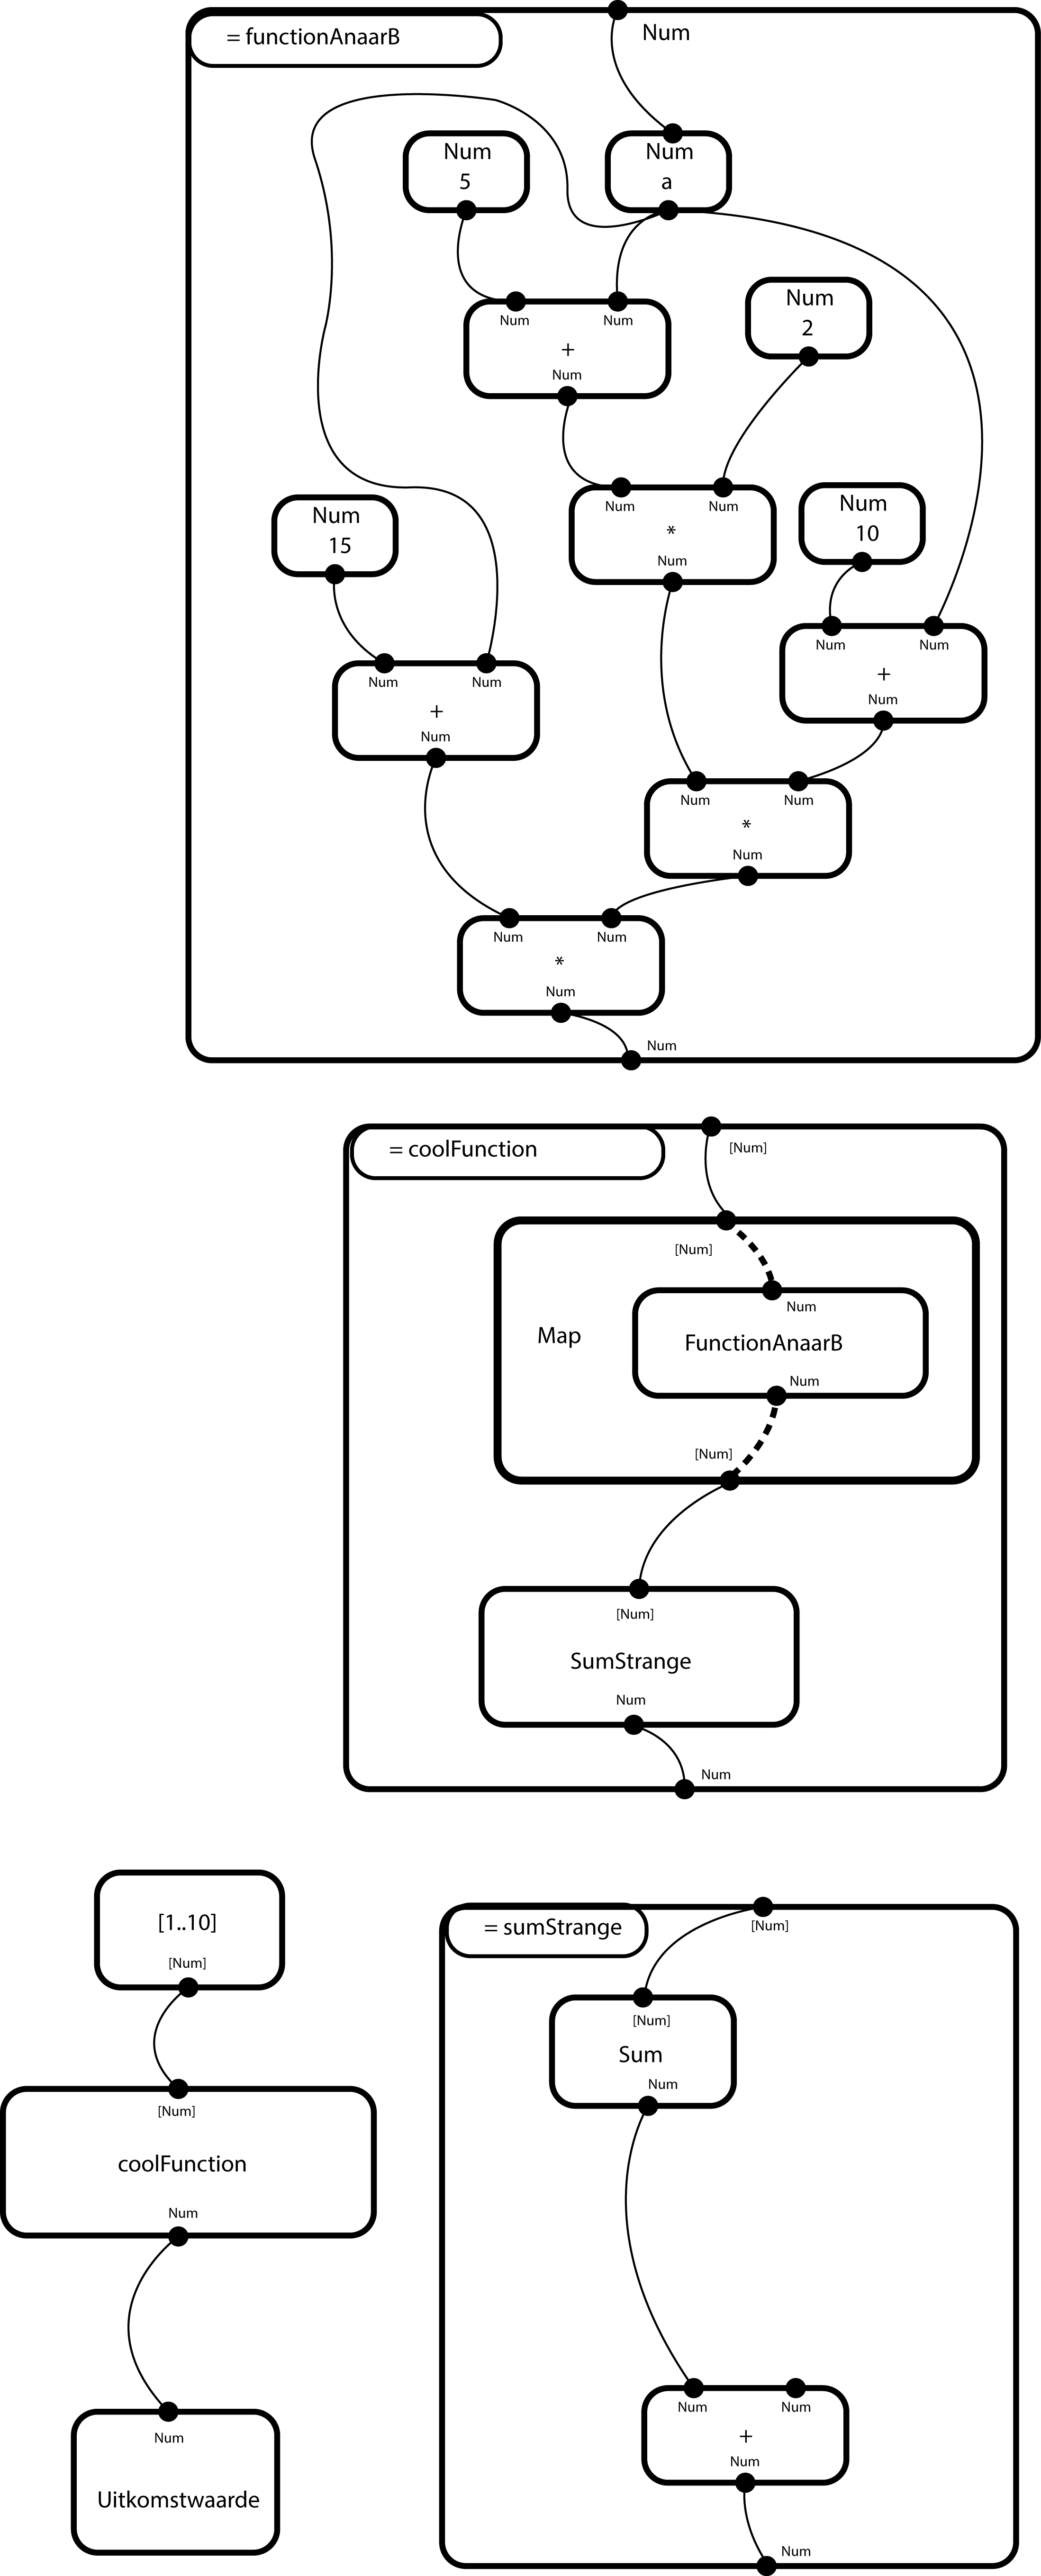
\includegraphics[scale=0.5]{Images/voorbeeldprogramma4.png}
	\label{fig:example-program-4}
	\caption{Dropped concept for representing functions.}
\end{figure}
\begin{figure}[p]
	\centering
	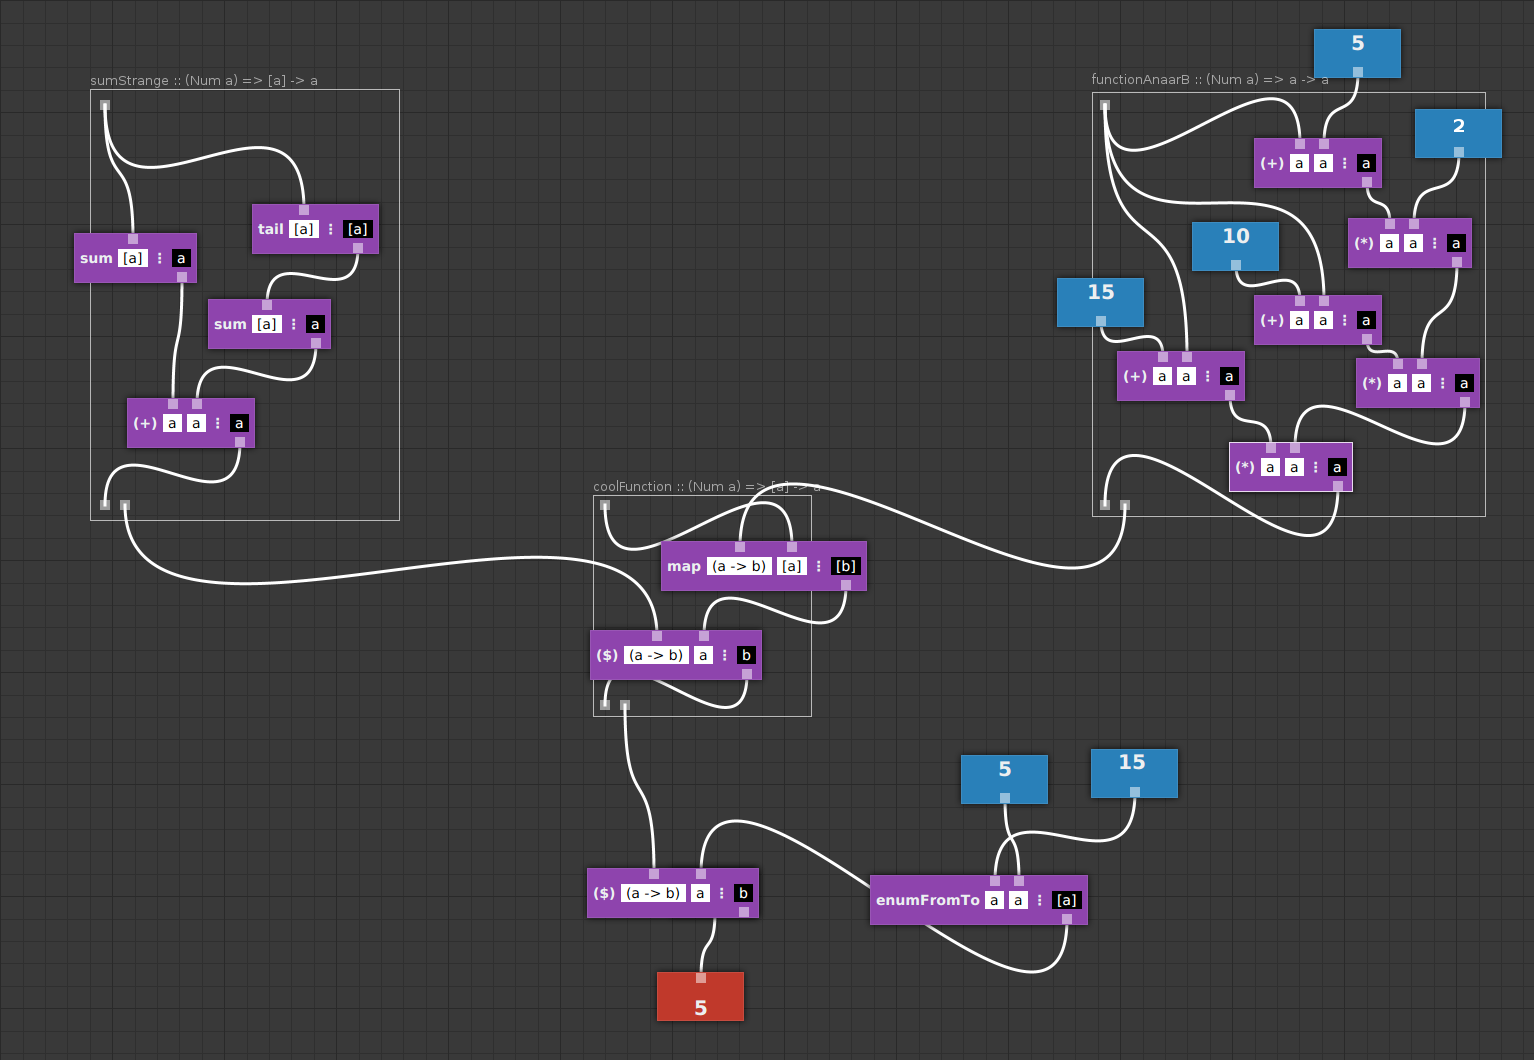
\includegraphics[scale=0.3]{Images/voorbeeldprogramma5.png}
	\label{fig:example-program-5}
	\caption{Concept of what turned into the final representation of functions.}
\end{figure}
